% remember to set these at the start of each chapter
\chapter{CNN architectures} 

%%%%%%%%%%%%%%%%%%
In this section, three CNN architectures are discussed. From a simple five-layer CNN, then a deeper 19-layer CNN VGG19, to a highly advanced CNN with shortcut connections Resnet.

\section{Small CNN}
Small CNN architecrure is dirived from \cite{Dhindsa2018}, which were used in grading the servery of prenatal hydronephrosis (PHN). Small CNN has five convolutional layer, followed by a fully connected layer of 512 units and an output layer. Each layer (convolutional and fully connected) uses units with rectified linear (ReLU) activation functions. The output layer uses SoftMax activation function for classification. 

The first convolutional layer contains 16 filters with an input patch of 7x7 pixels. The second layer has 32 filters and an input patch size of 5x5 pixels. The following three convolutional layers contain 64 filters with patch size of 3x3 pixels. A stride is set to 1 in all convolutional layers. Padding is set to ‘same’, which results in padding the input such that the output has the same length as the original input.

Each convolutional layer is followed by a max pooling layer with 3x3 patch with a stride of 2x2 pixels (a stride less than the pooling patch size has been demonstrated to improve DCNN performance for some computer vision tasks [12]). Pooling integrates the learned features in local patches and reduces the size of the image for subsequent layers. 

In addition to data augmentation, to reduce over fitting, batch normalization was performed after each convolutional layer, which normalizes the statistics of activations in a layer after a batch of images. In order to make training more robust and efficient, dropout is added after the fully connected layer to reduce overfitting and to promote learning more independent features.

\section{VGG}
VGG\citep{vgg} is a ConvNet architecture that has significantly higher accuracy than prior ConvNets. It achieved the state-of-the-art accuracy on ILSVRC 2015 classification and localisation tasks. 

The image is passed through a stack of convolutional layers. The filter that is used has a very small receptive field: 3 x 3 (which is the smallest size to capture the notion of left/right, up/down, center). Padding is set to "same". The convolution stride is 1. A max-pooling layer is added after two convolution layers for the first two blocks. For the third, fourth and fifth block, the setup is four convolution layers then max-pooling layer. All max-pooling is performed over a 2 x 2 pixel window, with stride 2x2 pixels. A stack of convolutional and max-pooling blocks is followed by three Fully-Connected (FC) layers: the first two have 4096 channels each, the third performs classification.All hidden layers are equipped with the rectification (ReLU) activation function. The final layer is Softmax for classification. Dropout layers are added between two FC layers. Dropout rate is set to 0.5. Fig.\,\ref{VGG} shows a VGG19 architecture.

\begin{figure}[h]
	\centering
	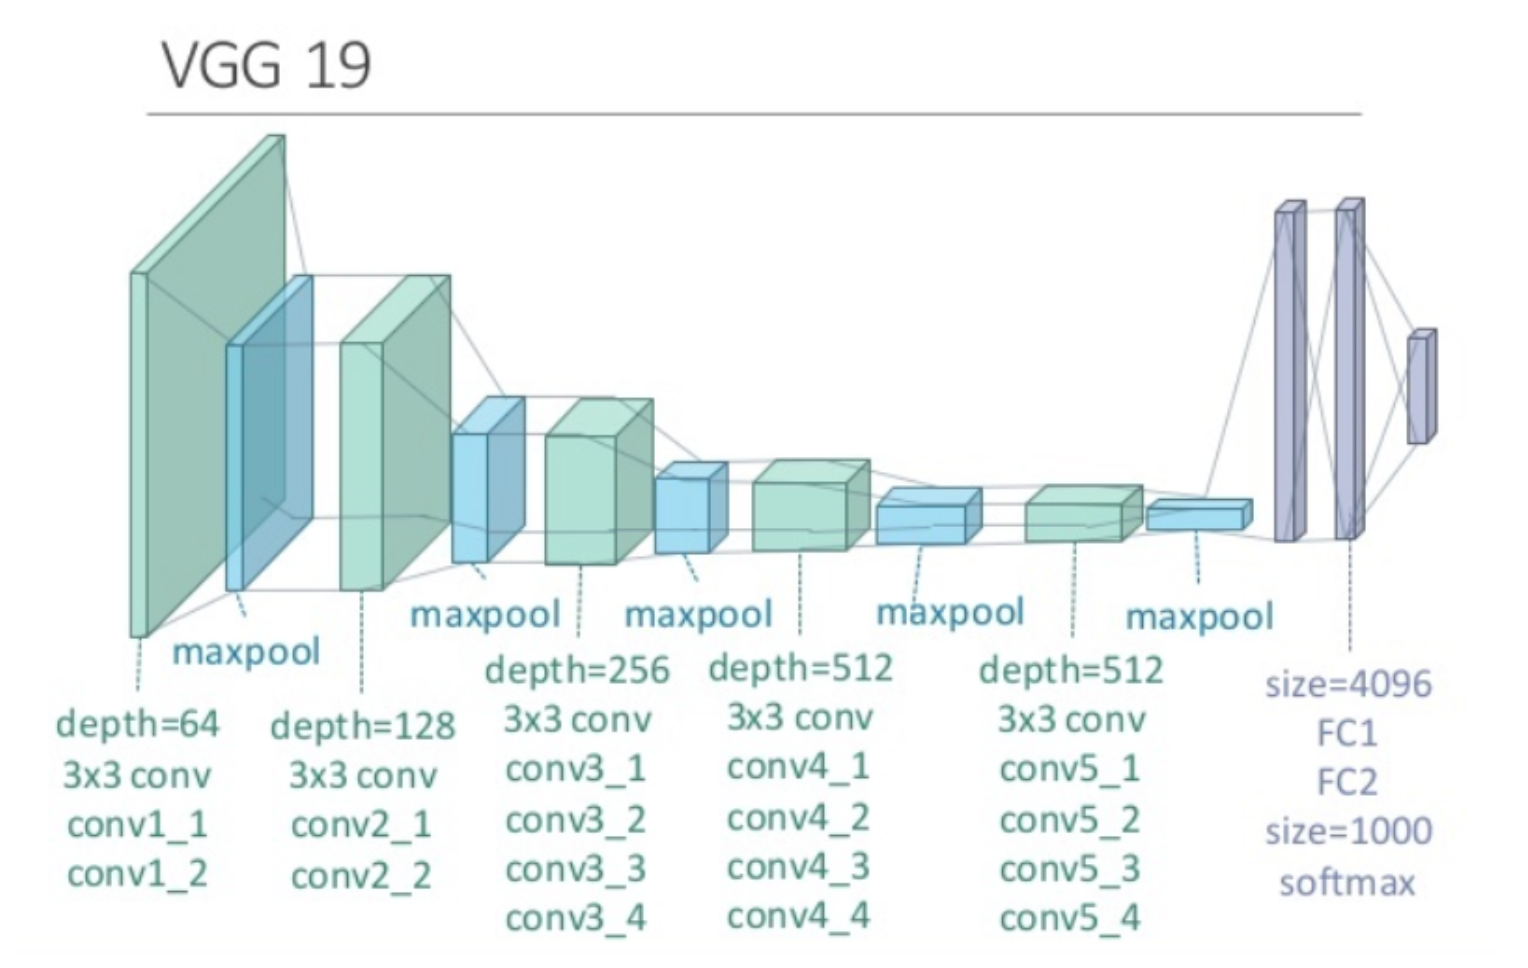
\includegraphics[width=\textwidth]{Figs/vgg.png}
    \caption{VGG19 architecture}
    \label{VGG}
\end{figure}

Rather than using relatively large receptive fields in the first convolutional layers, VGG uses very small 3 x 3 receptive fields throughout the whole net, which are convolved with the input at every pixel (with stride 1). However, the receptive field of a stack of two 3 x 3 conv. layers (without spatial pooling in between) is the same as that of 5 x 5; three 3 x 3 layers has the effective receptive field as 7 x 7. 

Comparing to a single 7 x 7 convolution layer, a stack of three 3 x 3 convolution layers give the benefit of incorporating three non-linear rectification layers instead of a single one, which makes the decision function more discriminative. Also, the number of parameter is decreased. A stack of three 3 x 3 filters have $3\times3^2 = 27$ parameters whereas a 7 x 7 filter has $7^2 = 49$ parameters. This can be seen as imposing a regularization on the 7 x 7 conv. filters, forcing them to have a decomposition through the 3 x 3 filters (with non-linearity injected in between).


\section{ResNet}

The depth of a neural network is an important factor influencing its performance. The architecture used in visual tasks is often very deep. We usually achieve better accuracy with deeper neural networks. However, when the network is too deep, we may encounter the vanishing gradient problem. In back-propagation, each of the neural network's weights receives an update proportional to the partial derivative of the error function with respect to the current weight in each iteration of training. In some cases, the gradient will be vanishingly small, effectively preventing the weight from changing its value. In the worst case, this may completely stop the neural network from further training. We can address this problem by normalized initialization [23, 9, 37, 13] and intermediate normalization layers, which enable networks with tens of layers to start converging for stochastic gradient descent (SGD) with backpropagation. 

When deeper networks are able to start converging, a degradation problem rises. Accuracy gets saturated sooner with the network depth increases. From \citeauthor{Srivastava2015}'s experiments\cite{Srivastava2015}  (Fig.\,\ref{deeploss}), the more layers in a deep neural network model, the higher the training error is. Such degradation is not caused by overfitting.

\begin{figure}[h]
	\centering
	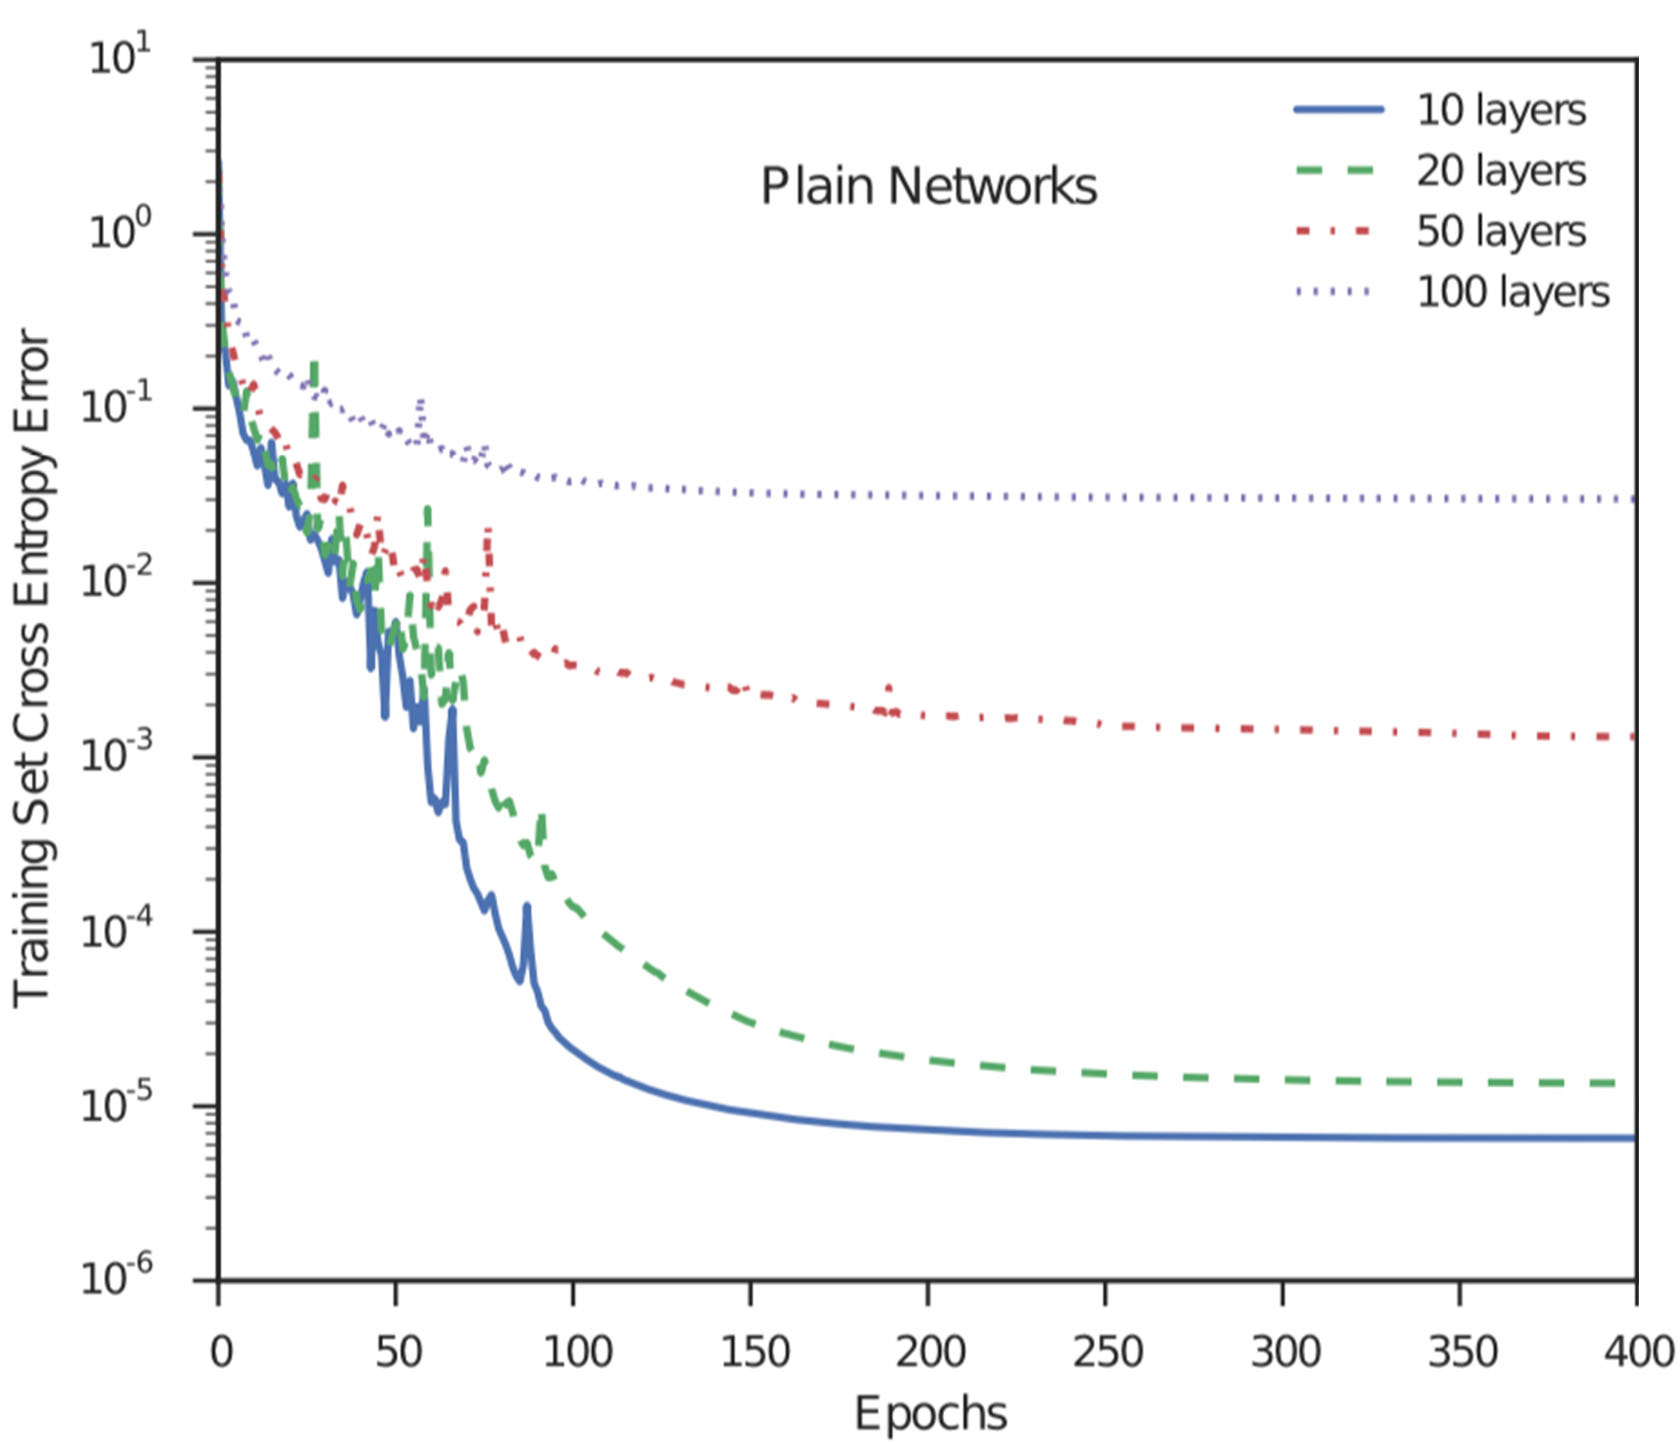
\includegraphics[scale=0.5]{Figs/deeploss.jpg}
    \caption{Training Loss: Deep vs. Shallow\cite{Srivastava2015}}
    \label{deeploss}
\end{figure}

The degradation (of training accuracy) indicates that not all systems are similarly easy to optimize. Let us consider a shallower architecture and its deeper counterpart that adds more layers onto it. There exists a solution by construction to the deeper model: the added layers are identity mapping, and the other layers are copied from the learned shallower model. The existence of this constructed solution indicates that a deeper model should produce no higher training error than its shallower counterpart. But experiments show that current solvers on hand are unable to find solutions that are comparably good or better than the constructed solution (or unable to do so in feasible time). 

The degradation problem is addressed by ResNet. In ResNet, the stacked layers fit a residual mapping, instead of fitting the whole desired underlying mapping. Formally, denoting the desired underlying mapping as $\mathcal{H}(\mathbf{x})$, let the stacked nonlinear layers fit another mapping of $\mathcal{F}(\mathbf{x}) := \mathcal{H}(\mathbf{x})-\mathbf{x}$. The original mapping is recast into $\mathcal{F}(\mathbf{x})+\mathbf{x}$. It is easier to optimize the residual mapping than to optimize the original, unreferenced mapping. To the extreme, if an identity mapping were optimal, it would be easier to push the residual to zero than to fit an identity mapping by a stack of nonlinear layers. 
\begin{figure}[h]
	\centering
	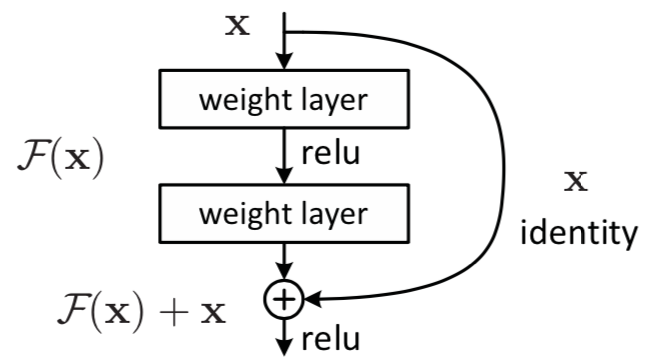
\includegraphics[scale=0.5]{Figs/residualblock.png}
    \caption{Residual learning: a building block  \cite{resnet}}
    \label{residualblock}
\end{figure}

The formulation of $\mathcal{F}(\mathbf{x})+\mathbf{x}$ can be realized by feedforward neural networks with “shortcut connections” (Fig.\,\ref{residualblock}). Shortcut connections [2, 34, 49] are those skipping one or more layers. In ResNet, the shortcut connections simply perform identity mapping, and their outputs are added to the outputs of the stacked layers (Fig.\,\ref{residualblock}). Identity shortcut connections add neither extra parameter nor computational complexity. The entire network can still be trained end-to-end by SGD with backpropagation, and can be easily implemented using common libraries without modifying the solvers. 

ResNet is concluded from experiments that "1) The extremely deep residual nets are easy to optimize, but the counterpart “plain” nets (that simply stack layers) exhibit higher training error when the depth increases; 2) Deep residual nets can easily enjoy accuracy gains from greatly increased depth, producing results substantially better than previous networks." \cite{resnet}

Residual Learning:
Let $\mathcal{H}(\mathbf{x})$ denote an underlying mapping to be fit by a few stacked layers (not necessarily the entire net), with $\mathbf{x}$ denoting the inputs to the first of these layers. If one hypothesizes that multiple nonlinear layers can asymptotically approximate complicated functions, then it is equivalent to hypothesize that they can asymptotically approximate the residual functions, i.e., $\mathcal{H}(\mathbf{x}) - \mathbf{x}$ (assuming that the input and output are of the same dimensions). So rather than expect stacked layers to approximate $\mathcal{H}(\mathbf{x})$, we explicitly let these layers approximate a residual function $\mathcal{F}(\mathbf{x}) := \mathcal{H}(\mathbf{x})-\mathbf{x}$. The original function thus becomes $\mathcal{F}(\mathbf{x})+\mathbf{x}$. Although both forms should be able to asymptotically approximate the desired functions (as hypothesized), the ease of learning might be different. 
This reformulation is motivated by the counter-intuitive phenomena about the degradation problem. If the added layers can be constructed as identity mappings, a deeper model should have training error no greater than its shallower counterpart. The degradation problem suggests that the solvers might have difficulties in approximating identity mappings by multiple nonlinear layers. With the residual learning reformulation, if identity mappings are optimal, the solvers may simply drive the weights of the multiple nonlinear layers toward zero to approach identity mappings. 
In real cases, it is unlikely that identity mappings are optimal, but our reformulation may help to precondition the problem. If the optimal function is closer to an identity mapping than to a zero mapping, it should be easier for the solver to find the perturbations with reference to an identity mapping, than to learn the function as a new one. We show by experiments (Fig. 7) that the learned residual functions in general have small responses, suggesting that identity map- pings provide reasonable preconditioning. 

Identity Mapping by Shortcuts: 
We adopt residual learning to every few stacked layers. A building block is shown in Fig.\,\ref{residualblock}. Formally, we define a building block as: 
\begin{equation} \label{eq1}
\mathbf{y} = \mathcal{F} (\mathbf{x}, \{W_i\}) + \mathbf{x}
\end{equation}

Here x and y are the input and output vectors of the layers considered. The function $\mathcal{F} (\mathbf{x}, \{W_i\})$ represents the residual mapping to be learned. For the example in Fig.\,\ref{residualblock} that has two layers, $\mathcal{F}=W_2\sigma(W_1\mathbf{X})$ in which $\sigma$ denotes ReLU activation function and the biases are omitted for simplifying notations. The operation $\mathcal{F} + \mathbf{x}$ is performed by a shortcut connection and element-wise addition. We adopt the second nonlinearity $\sigma(\mathbf{y})$ after the addition. The shortcut connections in Equation(\ref{eq1}) introduce neither extra parameter nor computation complexity. This is not only attractive in practice but also important in our comparisons between plain and residual networks. We can fairly compare plain/residual networks that simultaneously have the same number of parameters, depth, width, and computational cost (except for the negligible element-wise addition). 
The dimensions of $\mathbf{x}$ and $\mathcal{F}$ must be equal in Equation(\ref{eq1}). If this is not the case (e.g., when changing the input/output channels), we can perform a linear projection $W_s$ by the shortcut connections to match the dimensions: 

\begin{equation} \label{eq2}
\mathbf{y} = \mathcal{F} (\mathbf{x}, \{W_i\}) + W_s \mathbf{x}
\end{equation}

We can also use a square matrix $W_s$ in Equation(\ref{eq1}). But we will show by experiments that the identity mapping is sufficient for addressing the degradation problem and is economical, and thus $W_s$ is only used when matching dimensions. 

Although the above notations and equations only demonstrate fully-connected layers for simplicity, they are also applicable to convolutional layers. The function $\mathcal{F} (\mathbf{x}, \{W_i\})$ can represent multiple convolutional layers. The elementwise addition is performed on two feature maps.

Network Architecture:
We have two types of ResNet block, depending on whether the input/output dimensions are same or different.

\begin{figure}[h]
	\centering
	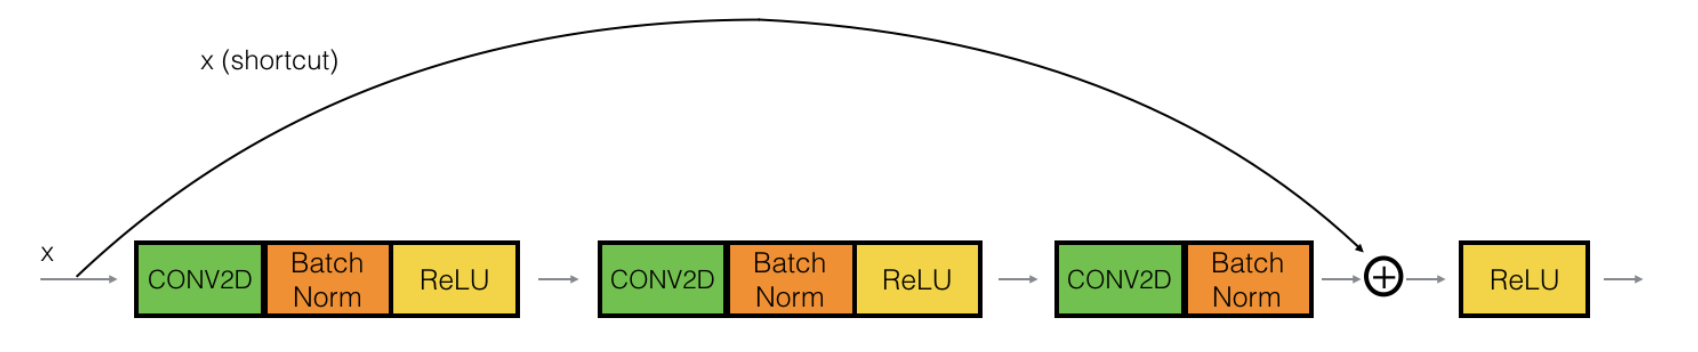
\includegraphics[width=\textwidth]{Figs/identityblock.png}
    \caption{Identity Block}
    \label{identityblock}
\end{figure}

\begin{enumerate}
\item  \textbf{Identity block} (Fig.\,\ref{identityblock}) is the standard block used in ResNets, and corresponds to the case where the input activation has the same dimension as the output activation (Equation(\ref{eq1})).
    \begin{description}
      \item[$\ast$ First component of main path:] The first CONV2D has $F_1$ filters of shape (1,1) and a stride of (1,1). Its padding is "valid", which means no padding. The first BatchNorm is normalizing the channels axis. Then apply the ReLU activation function. 
      \item[$\ast$ Second component of main path:] The second CONV2D has $F_2$ filters of shape $(f,f)$ and a stride of (1,1). Its padding is "same", meaning the output is padded to the same size of input. The second BatchNorm is normalizing the channels axis. Then apply the ReLU activation function. 
      \item[$\ast$ Third component of main path:] The third CONV2D has $F_3$ filters of shape (1,1) and a stride of (1,1). Its padding is "valid". The third BatchNorm is normalizing the channels axis. Note that there is no ReLU activation function in this component.
      \item[$\ast$ Shortcut path:] Shortcut path is just simply the input.
      \item[$\ast$ Final step:] The shortcut and the input are added together. Then apply the ReLU activation function.
    \end{description}
    
\begin{figure}[h]
\centering
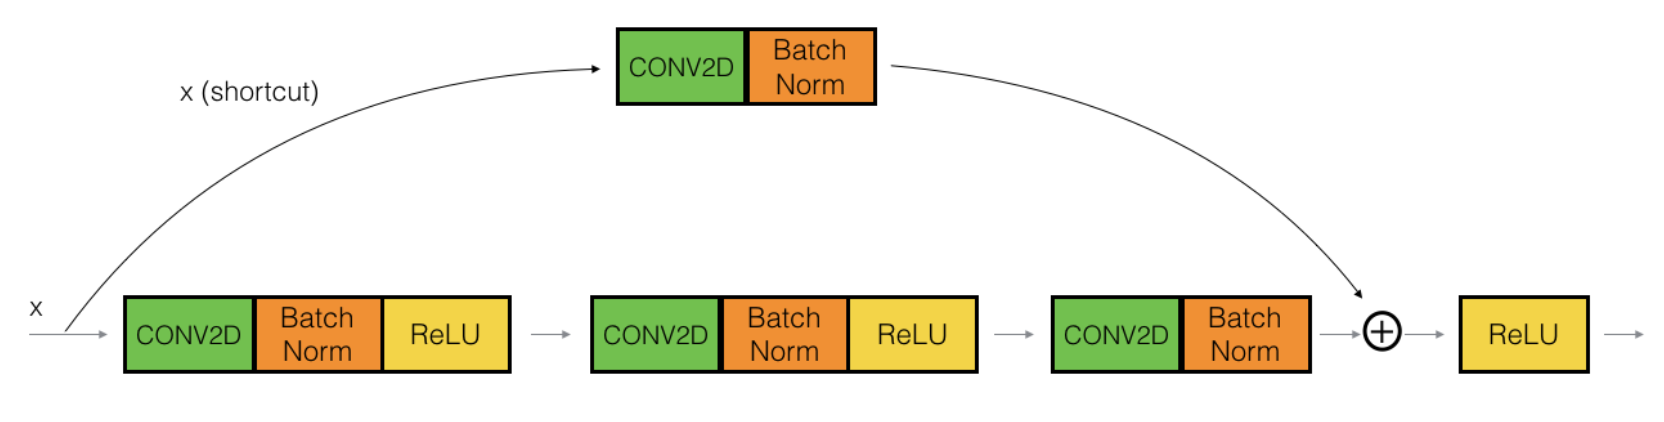
\includegraphics[width=\textwidth]{Figs/convolutionblock.png}
\caption{Convolutional Block}
\label{convolutionblock}
\end{figure}

\item  \textbf{Convolutional Block} is used when the input and output dimensions don't match up. The only difference comparing to identity block is that convolutional block has a convolutional layer in the shortcut path to match the dimensions (Equation(\ref{eq2})).
    \begin{description}
      \item[$\ast$ First component of main path:] The first CONV2D has $F_1$ filters of shape (1,1) and a stride of $(s,s)$. Its padding is "valid". The first BatchNorm is normalizing the channels axis. Then apply the ReLU activation function. 
      \item[$\ast$ Second component of main path:] The second CONV2D has $F_2$ filters of shape $(f,f)$ and a stride of (1,1). Its padding is "same". The second BatchNorm is normalizing the channels axis. Then apply the ReLU activation function. 
      \item[$\ast$ Third component of main path:] The third CONV2D has $F_3$ filters of shape (1,1) and a stride of (1,1). Its padding is "valid". The third BatchNorm is normalizing the channels axis. There is no ReLU activation function.
      \item[$\ast$ Shortcut path:] The CONV2D has $F_3$ filters of shape (1,1) and a stride of $(s,s)$. Its padding is "valid". The BatchNorm is normalizing the channels axis. 
      \item[$\ast$ Final step:] The shortcut and the input are added together. Then apply the ReLU activation function.
    \end{description}
\end{enumerate}

Resnet-18 architecture is built as the following:

\textbf{Stage 1}:
Zero-padding pads the input with a pad of (3, 3)
Convolution layer has 64 filters of shape (7, 7) and uses a stride of (2, 2).
BatchNorm is applied to the channels axis of the input.
MaxPooling uses a (3, 3) window and a (2, 2) stride.

\textbf{Stage 2}:
One convolutional block uses three set of filters $(F_1=F_2=F_3)$ of size [64, 64, 256], filter shape $f$ set to 3, stride $s$ set to 1.
Two identity blocks use three set of filters $(F_1=F_2=F_3)$ of size [64, 64, 256], filter shape $f$ set to 3.

\textbf{Stage 3}:
One convolutional block uses three set of filters of size [128, 128, 512], $f$ is 3, $s$ is 2.
Two identity blocks use three set of filters of size [64, 64, 256], $f$ is 3.

\textbf{Stage 4}:
One convolutional block uses three set of filters of size [256, 256, 1024], $f$ is 3, $s$ is 2.
Two identity blocks use three set of filters of size [256, 256, 1024], $f$ is 3.

\textbf{Stage 5}:
One convolutional block uses three set of filters of size  [512, 512, 2048], $f$ is 3, $s$ is 2.
Two identity blocks use three set of filters of size  [512, 512, 2048], $f$ is 3.

\textbf{Stage 6}:
One 2D Average Pooling uses a window of shape (2,2).
A flatten layer.
Finally, a Fully Connected (Dense) layer reduces its input to the number of classes (2 in this case) using a softmax activation.
